
\begin{frame}{LMM (unequal variance)}
	\begin{minipage}{.45\linewidth}
		\begin{center}
			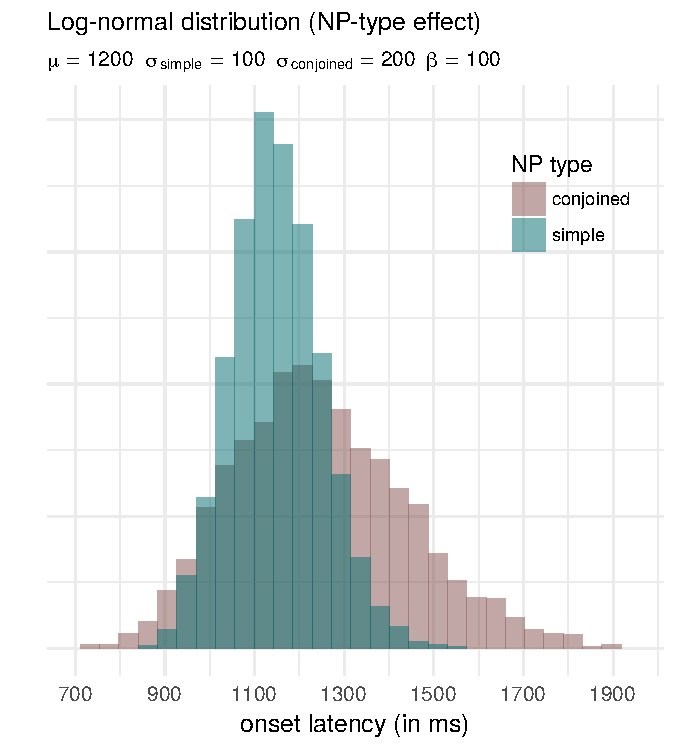
\includegraphics[scale=.4]{gfx/unequalvar.pdf}
		\end{center}
	\end{minipage}
	\hfill
	\begin{minipage}{.5\linewidth}
		\begin{footnotesize}
			The conjoined NP condition has a larger variance than the simple NP condition: $\sigma_{e''}^2 > \sigma_{e'}^2$.
		\end{footnotesize}
			
		\begin{tiny}
			\begin{equation}
			y_{i} \sim
			\begin{cases} 
			LogNormal(\mu, \sigma_{e'}^2) \text{, if } NP_i = simple\\
			LogNormal(\mu + \beta, \sigma_{e''}^2) \text{, else if } NP_i = conjoined
			\end{cases}
			\end{equation}
		\end{tiny}
			
	
	\end{minipage}
	
\end{frame}

